\setcounter{chapter}{2}
\setcounter{section}{0}
\setcounter{figure}{0}
\setcounter{equation}{0}
\setcounter{table}{0}
\chapter*{
\includegraphics[width=\textwidth]{./figures/Topic2/Topic2.jpg}}
\addcontentsline{toc}{chapter}{Topic 2: Fluid Mechanics of the Circulatory System}

\section{Introduction}

Single-cell organisms live in direct contact with the environment from where they derive nutrients and into where they dispose of their waste. For living systems containing multiple cells, there is the challenge of how to get nutrients past multiple layers of cells efficiently and how to avoid the build-up in waste products within deep cellular layers. The answer to these challenges is the development of an intricate plumbing network, containing pumps and distribution lines that are collectively called the circulatory system.  

\begin{wrapfigure}{r}{0.5\textwidth} 
\vspace{-20pt}
  \begin{center}
    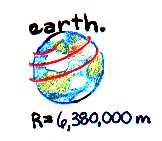
\includegraphics[width=0.4\textwidth]{./figures/Topic2/Earthclip.jpg}
    %\caption{}
%    \label{fig:databaseUserTable}
  \end{center}
  \vspace{-20pt}
  \vspace{1pt}
\end{wrapfigure} 
To give you a sense for the complexity of the human circulatory system consider the following facts. Lined up end-to-end, your blood vessels would wrap more than twice around the Earth, and your circulatory system pumps over five liters of blood through the body every minute.  Meandering through vast networks of capillaries, blood delivers oxygen and nutrients to the body’s cells at a leisurely 0.026cm/s.  In contrast, it rushes through the aorta at 30cm/s, over a thousand times faster.
 
The pressure in the circulatory system also undergoes changes as it traverses blood vessels of differing diameters and as it defies or succumbs to gravity.  Thus as we shall see, pressure is usually higher in the arteries than in the veins, but it also varies with posture. This is why accident victims are directed to keep bleeding wounds raised above heart level; this action lowers the blood pressure in the wound, and consequently lessens the bleeding.  
Applying the laws of fluid mechanics to blood flow not only helps us understand the factors governing circulation, but lets us design better medical instruments and more effective treatments for diseases and accidents involving the circulation.  

\section{Fluid Dynamics of Human Circulation}

\subsection{Pressure and flow rate along a pipe: a few fundamental concepts} 

A fluid can move one way inside a pipe only if the fluid is pushed with a greater force from one side than from the other, i.e. if a pressure difference exists between the ends of the pipe. For example, when one end of a hose is connected to a faucet and the other placed over a drain, the water inside the hose experiences a pressure difference. That is, the side connected to the faucet is subjected to a high pressure (typically 60 PSI) whereas the side that empties into the drain is at 0 PSI. The pressure inside the hose varies accordingly from 60 PSI for a point near the faucet to 0 PSI at another point near the drain. In between, the pressure varies gradually between those two extremes (see Fig.~\ref{Fig2-1}).
\begin{figure}[htb]
	\centering
	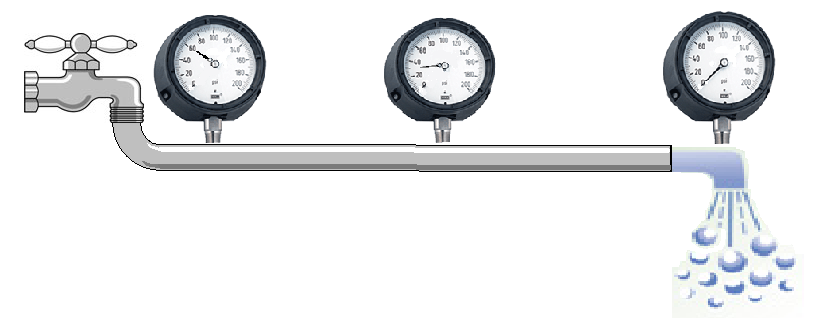
\includegraphics[width=\textwidth]{./figures/Topic2/Fig2-1.png}
	\caption{Pressure drops gradually but flow rate remains the same throughout the pipe.}
	\label{Fig2-1}
\end{figure}

The fluid flow rate, i.e. the volume of fluid flowing through the hose per unit time (e.g. gallons,/min or cc/min), is directly proportional to the pressure difference across the ends. Unlike pressure, which drops gradually along the length of the hose, the flow rate at any point is always the same. That is, what goes into the hose in a given amount of time must come out over the same time. This is simply a reflection of conservation of mass. Were this not the case, mass would accumulate or vanish within the pipe. 

The system depicted in Fig.\ref{Fig2-1} is an example of an open system, i.e. one where the fluid is lost at the drain side. Obviously this is not a desirable design for a circulatory system where blood must be preserved. A closed system, i.e. one where blood is recycled back into the starting point, is thus absolutely necessary for the function of an animal. To accomplish this, a pump must exist to recycle the fluid back and to pressurize it once more so that its flow is maintained constant throughout the system. The heart fulfills that function. 

\subsection{The Systemic and Pulmonary Systems}

In addition to the need for a pump, the circulatory system requires constant intaking of oxygen and expelling of carbon dioxide that accumulates from metabolic processes. This gas exchange function is performed by the lungs, an organ that must therefore be an integral part of the circulatory system as important as the heart. 

The need to enrich blood with oxygen before delivering it to the body poses an interesting hydrodynamic challenge for the circulatory system that is illustrated in Fig.~\ref{Fig2-2}(a). Fish employ such a simple design. As blood traverses the network of capillaries within the gills it loses much pressure, but enough remains to push blood at rates that meet the fish’s demand for oxygen. Mammals, however, have much higher metabolic rates and thus must consume more oxygen. The pressure out of the lungs would be insufficient to push blood at rates needed to deliver sufficient oxygen for the rest of the body. To circumvent this problem, animals have evolved a circulatory system that includes the dual pumping system illustrated in Fig.~\ref{Fig2-2}(b). The second pump increases the pressure to a level sufficient to push blood throughout the body. 
\begin{figure}[htb]
	\centering
	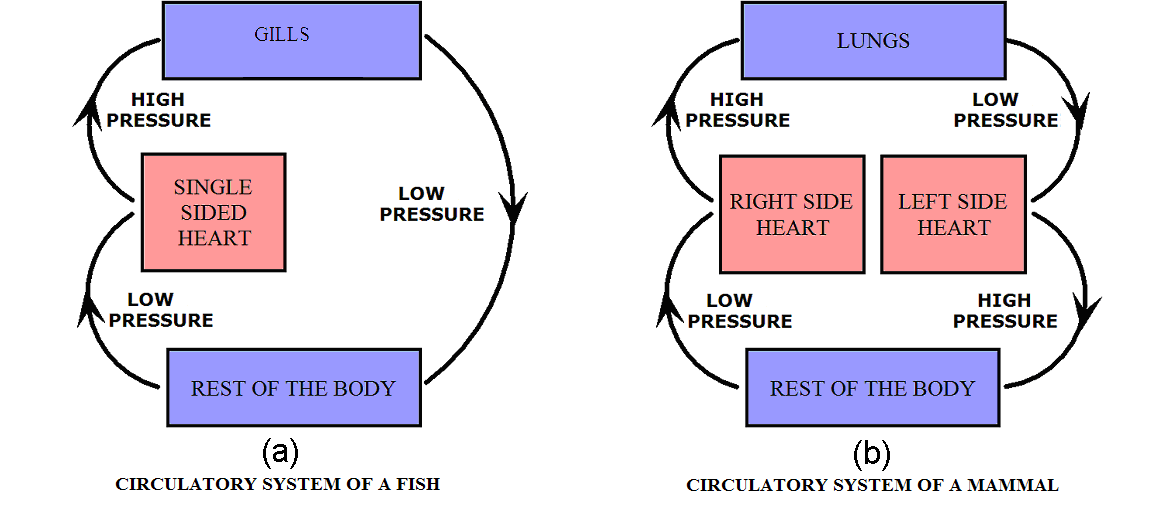
\includegraphics[width=\textwidth]{./figures/Topic2/Fig2-2.png}
	\caption{Diagram of flow through air intake and the rest of the body. High and low pressure areas are indicated.}
	\label{Fig2-2}
\end{figure}

The mammalian heart has four chambers, allowing it to serve as a pump for two distinct circuits: the pulmonary system, which pumps blood through the lungs, and the systemic system, which services the rest of the body.  Two of the chambers, called atria, collect blood entering the heart and pump it to the other two chambers, called ventricles, which pump it throughout the body.  (See Figure \ref{Fig2-3}.)  In the pulmonary circuit, blood leaves the right ventricle via the pulmonary arteries and passes through capillary beds in the lungs, where carbon dioxide is exchanged for oxygen.  The oxygen-rich blood then returns to the heart, moving through the pulmonary veins to the left atrium.  Next it flows to the left ventricle, where it is forcefully pumped through the aorta to the rest of the body.  Two large veins called vena cavae (superior and inferior) collect the oxygen-poor blood and return it to the heart, depositing it in the right atrium.  
\begin{figure}[htb]
	\centering
	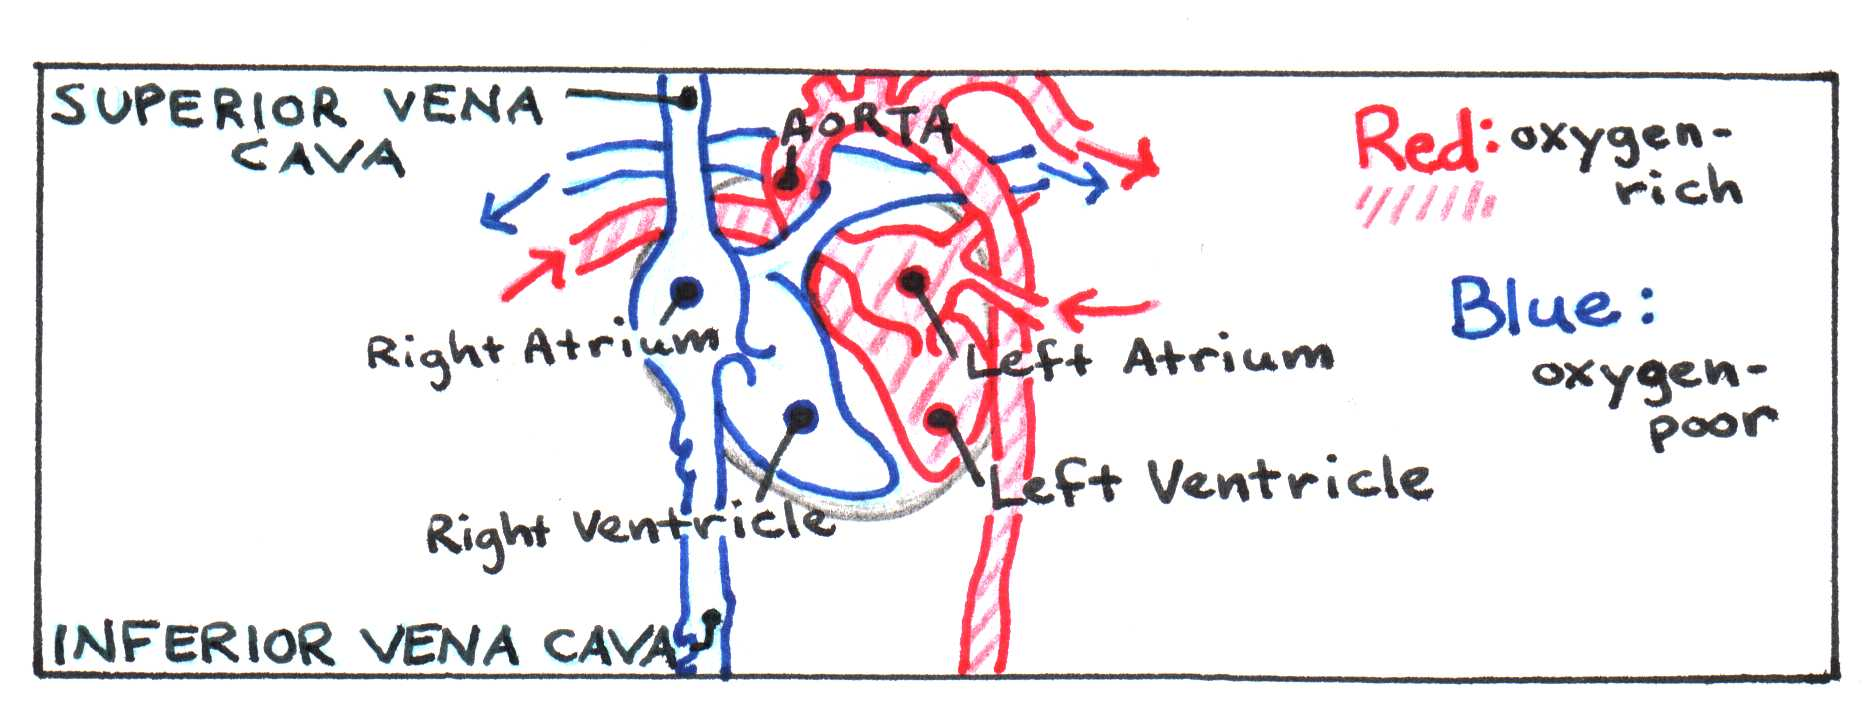
\includegraphics[width=\textwidth]{./figures/Topic2/Fig2-3.jpg}
	\caption{Diagram of flow through the heart.}
	\label{Fig2-3}
\end{figure}  

In either system, arteries carry blood away from the heart, branching into smaller blood vessels called arterioles.  These branch further into microscopic capillaries that network through tissues, allowing chemical exchange to occur.  Downstream of capillary beds, the capillaries converge into venules, which in turn converge into veins.  Veins bring blood back to the heart, completing the circuit.

In both the systemic and pulmonary systems, valves in the heart allow pressure to build before the blood is pumped out of the heart.  Blood travels further in the systemic system than in the pulmonary system, so pressure in the aorta must be much greater than in the pulmonary arteries.  Figure \ref{Fig2-4} illustrates the pressure differences in the different parts of the circulatory system.
\begin{figure}[htb]
	\centering
	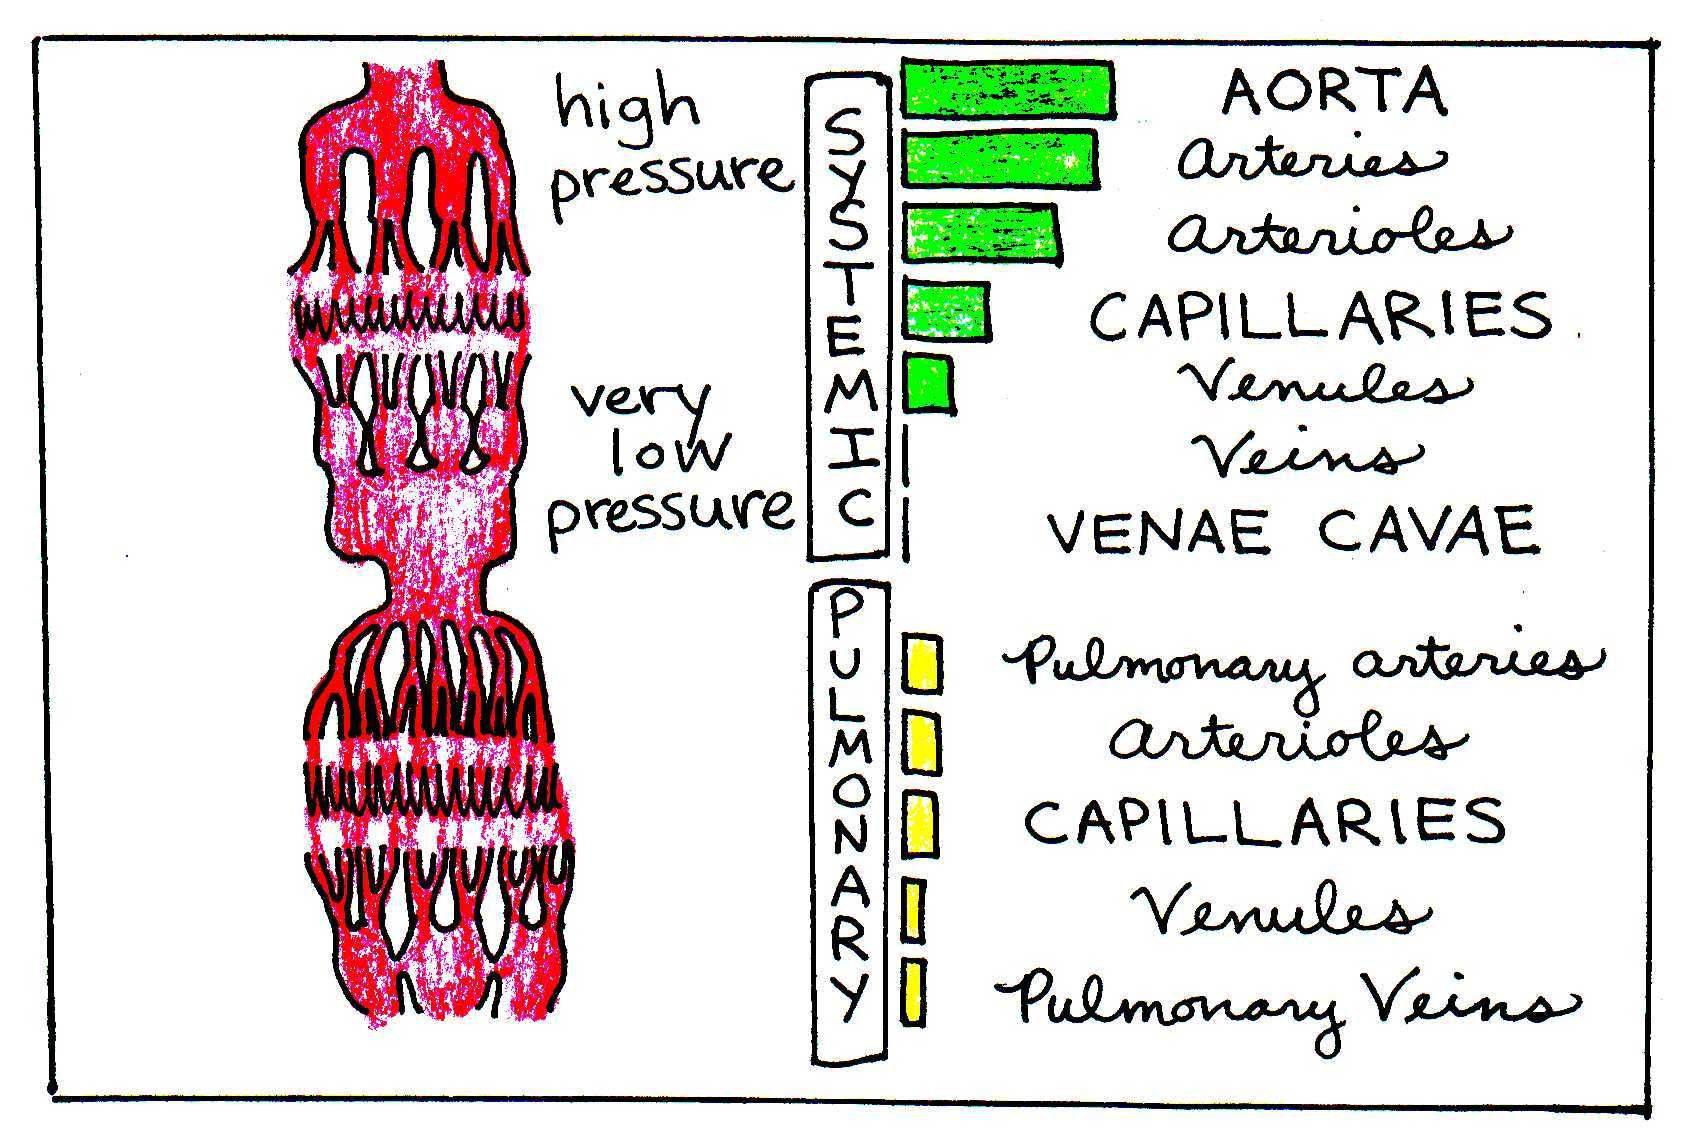
\includegraphics[width=\textwidth]{./figures/Topic2/Fig2-4.jpg}
	\caption{The green and yellow bars illustrate the varying levels of blood pressure in the different portions of the circulatory system.}
	\label{Fig2-4}
\end{figure}

\subsection{The Continuity Equation}

The volume flow rate through a pipe is defined as the volume of the fluid that passes a particular point per unit time.  We can quantify it by multiplying the cross-sectional area $A$ of the pipe by the velocity of the fluid $v$, which is distance covered per unit time. This is diagrammed in Fig.~\ref{Fig2-5}.
\begin{figure}[htb]
	\centering
	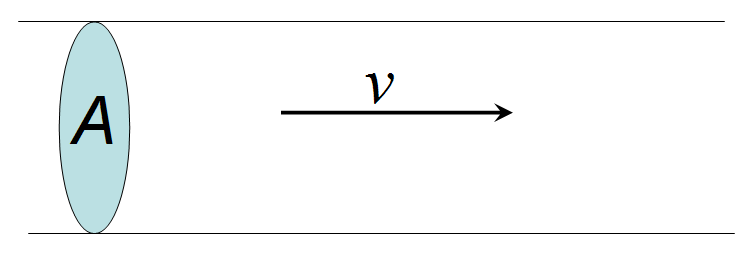
\includegraphics[width=3.5in]{./figures/Topic2/Fig2-5.png}
	\caption{Schematic of fluid flow at velocity, $v$ passing through a cross-sectional area, $A$.}
	\label{Fig2-5}
\end{figure}
\begin{equation}\label{eqn2-1}
\frac{dV}{dt} = Av
\end{equation}

Note that this gives the correct units of the flow rate: cm$^3$/s. Since blood is not compressible, volume is preserved unless there is a break in a blood vessel.  It follows, then, that the volume flow rate remains constant everywhere, since the flow is circular.  This means that a fluid moving through a wide vessel must move more quickly when the vessel narrows.  This relationship between cross-sectional area and velocity in different portions of the circulatory system is expressed by the continuity equation:
\begin{equation}\label{eqn2-2}
\frac{dV}{dt} = A_{aorta}v_{aorta} = A_{capillary}v_{capillary}
\end{equation}
where $A_{aorta}$ is the cross-section of the aorta and $A_{capillary}$ is the combined cross-section of all the capillaries. If we could lump all the blood vessels together by class, the circulatory system could be visualized as a pipe circuit, as in Figure \ref{Fig2-6}.
\begin{figure}[htb]
	\centering
	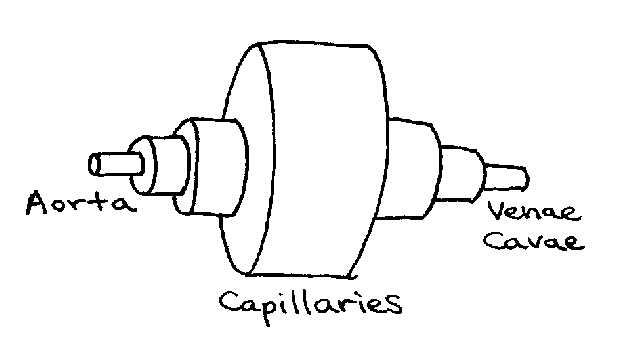
\includegraphics[width=4in]{./figures/Topic2/Fig2-6.jpg}
	\caption{Pipe circuit analogous to circulatory system. Note that each section represents the effective diameter of a particular type of vessel (e.g. capillaries) after all vessels of that type are combined.}
	\label{Fig2-6}
\end{figure}
Table \ref{table2-1} below gives the total cross-sectional area of the blood vessels within each part of the system.
\begin{table}[htb]
\begin{center}
\begin{tabular}{|l|c|}
\hline
Vessel & Area (cm$^2$) \\
\hline
aorta & 2.5 \\
small arteries & 20 \\
arterioles & 40 \\
capillaries & 2600 \\
venules & 250 \\
small veins & 80 \\
venae cavae & 8 \\
\hline
\end{tabular}
\caption{Total cross-sectional area of all blood vessels in humans.}
\label{table2-1}
\end{center}
\end{table}
The volume flow rate out of the heart into the aorta is roughly 80 ml/s.  By using this value and A = 2.5 cm$^2$ from Table 1, we use Eq.~(1) to calculate the corresponding velocity of blood in the aorta to be 32 cm/s.  Similarly, we can find the velocity of blood through the capillaries:  $dV/dt = 80 cm^3/s = A_{capillary}v_{capillary}$.  Using A = 2600 cm$^2$ from Table \ref{table2-1}, we find that $v_{capillaries}$ = 0.031 cm/s, roughly a thousand times slower than in the aorta.

Because of the inverse relationship between area and velocity in the continuity equation, we might be tempted to think that blood flows much faster through the tiny capillaries than through the huge veins and arteries.  This logic is misleading, however the total cross-sectional area is what matters, not the area of an individual blood vessel.

\subsection{Hydrostatics}
 
Fluid flow is described in general by Bernoulli's equation.
\begin{equation}\label{eqn2-3}
P_1 + \rho g y_1 + \frac{1}{2}\rho v_1^2 = P_2 + \rho g y_2 + \frac{1}{2}\rho v_2^2
\end{equation}
where the variables $P$, $y$, and $v$ represent the pressure, elevation, and velocity, respectively, of a fluid at a given point as shown below in Fig.~\ref{Fig2-7}.
\begin{figure}[htb]
	\centering
	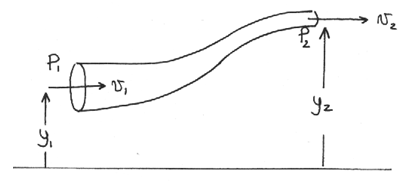
\includegraphics[width=\textwidth]{./figures/Topic2/Fig2-6.png}
	\caption{Diagram of a fluid flow tube with labels pertaining to Bernoulli's Equation.}
	\label{Fig2-7}
\end{figure}
When the velocity terms are negligible\footnote[2]{Proof is left as a homework assignment.}, as is often the case in the circulation, Eq.~\ref{eqn2-3} reduces to 
\begin{equation}\label{eqn2-4}
P_1 + \rho g y_1 = P_2 + \rho g y_2
\end{equation}
By combining the $\rho g y$ terms, the equation becomes even simpler.
\begin{equation}\label{eqn2-5}
P = P_{\circ}+ \rho g h,
\end{equation}
$P_{\circ}$ is the pressure at an arbitrary reference point (in our case, the heart), and $h = y_2-y_1$ is the depth of the fluid below that point. This equation reflects the well-known phenomenon of increased pressure with depth.  The mean arterial pressure for a human lying down is 100 mmHg (1 mmHg = 133 Pa). However, in an upright human, that arterial pressure can vary from 90 mmHg in the brain to 190 mmHg in the feet. The corresponding venous pressure can vary from -10 to 90 mmHg. These pressure values are relative to atmospheric pressure (i.e. gauge pressure).

\subsection{Effects of Viscosity}

Viscosity refers to the internal friction of a fluid resulting when layers of the fluid rub past each other.  This happens all the time inside pipes where layers adjacent to the walls move slower than layers deep inside the pipe.  Like any other frictional phenomenon, viscosity causes the fluid to gradually slow down.
Imagine standing on a bridge over a creek, dropping leaves into the water.  The leaves that fall near the center of the stream float along much faster than the ones that land near the water’s edge.  In the same way, blood at the center of a blood vessel moves at a higher velocity than it does along the walls.  It helps to think of the blood as being partitioned in concentric cylindrical layers, each moving at a slightly different speed.  Figure \ref{Fig2-8} illustrates this concept.  
\begin{figure}[htb]
	\centering
	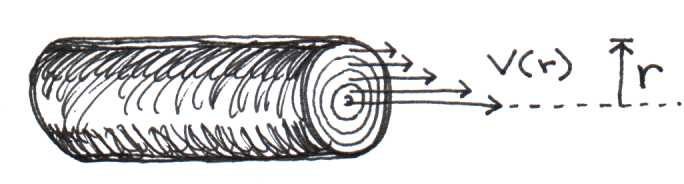
\includegraphics[width=4in]{./figures/Topic2/Fig2-7.jpg}
	\caption{Blood moves in concentric layers.  Layers closest to the center move fastest.}
	\label{Fig2-8}
\end{figure}
Viscosity arises because of the frictional force created between adjacent layers of the fluid that are moving at different speeds. The magnitude of the frictional force $F$ is directly dependent on the velocity difference $dv$ of the two layers separated by a distance $dr$, as well as the surface area of contact between them. The frictional force between two sheets is given by 
\begin{equation}\label{eqn2-6}
F = \eta A \frac{dv}{dr}
\end{equation}
where $\eta$ (greek letter ``eta'') is the viscosity and $A$ is the area of the common surface between layers.  In longer vessels, the effects of viscosity are more pronounced, because the common surface area between layers is increased. Calculations involving frictional forces are traditionally performed in the cgs (centimeters-grams-seconds) system of units, rather than in the SI system.  Thus, for example, the unit of force in the cgs system, called a dyne, is expressed in g$\cdot$cm/s$^2$ instead of kg$\cdot$m/s$^2$ for the Newton in the SI system. The unit of viscosity $\eta$ is called the poise, where 1 poise = 1 dyne$\cdot$s/cm$^2$. Table \ref{table2-2} is a set of conversions that you will find helpful when performing fluid calculations.
\begin{table}[h]
\begin{center}
\begin{tabular}{|l|l|l|}
\hline
Quantity & cgs & SI \\
\hline
Force & 1 dyne & 10$^{-15}$ Newtons (N) \\
Pressure & 10 dynes/cm$^2$ & 1 Pascal (N/m$^2$) \\
Pressure & 1 mmHg & 133 Pascal \\
Viscosity & 1 Poise (dyne$\cdot$s/cm$^2$)  & 0.1 kg/m$\cdot$s\\
\hline
\end{tabular}
\caption{Useful force, pressure, and viscosity conversions.}
\label{table2-2}
\end{center}
\end{table}

Viscosity depends on the nature of the fluid, but it can change with temperature.  Honey is highly viscous, but when heated in the microwave, it flows much faster out of the bottle.  As temperature increases, viscosity decreases.  Table \ref{table2-3} lists the viscosities for several fluids at different temperatures.  
\begin{table}[h]
\begin{center}
\begin{tabular}{|c|c|c|}
\hline
Fluid & Viscosity (poise) & Temperature ($^{\circ}$C) \\
\hline
water & 0.010 & 20 \\
water & 0.007 & 37 \\
blood plasma & 0.015 & 37 \\
whole blood & 0.040  & 37\\
thick oil & ~10 & 20 \\
\hline
\end{tabular}
\caption{Viscosity depends on temperature and can have a wide range of values depending on the nature of the fluid.}
\label{table2-3}
\end{center}
\end{table}
The blood viscosity shown in Table \ref{table2-2} is based on blood with a normal hematocrit (red blood cell content).  Abnormal hematocrits, such as those created by anemia or dehydration, can cause the blood viscosity to change dramatically.   Figure \ref{Fig2-9} illustrates how viscosity depends on the hematocrit. 
\begin{figure}[htb]
	\centering
	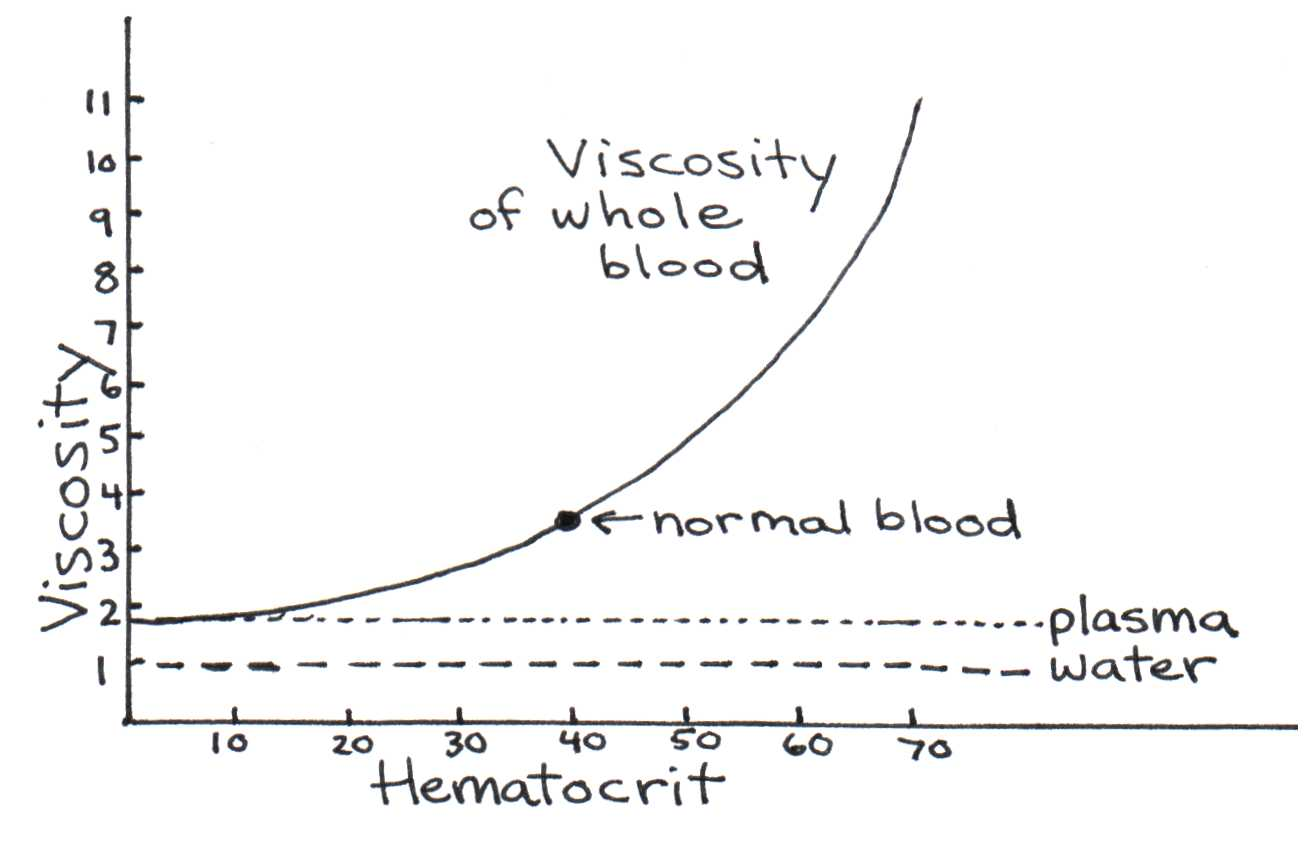
\includegraphics[width=\textwidth]{./figures/Topic2/Fig2-8.jpg}
	\caption{Viscosity’s dependence on the hematocrit.}
	\label{Fig2-9}
\end{figure}
Below a critical diameter of a blood vessel ($\sim$1.5 mm), red blood cells begin to align to pass through the vessel efficiently.  This causes the viscosity to decrease.  The viscosity then increases again in the capillaries, where red blood cells must squeeze through the tiny diameter.
As noted before, blood moves faster in the center of a blood vessel than near the walls.  How can we calculate the velocity of a layer of blood with radius $r$?  Consider a blood vessel of radius $R$ and of length $L$.  If blood is pushed into the vessel by a constant force $F$, we can integrate $dv$ from Eq.~\ref{eqn2-6} (see Appendix A)to show that 
\begin{equation}\label{eqn2-7}
v(r)=\Delta P\frac{R^2-r^2}{4\eta L}
\end{equation}
where $\Delta P$ is the pressure difference from one side of the tube to the other.  The velocity is greatest when $r$ = 0, at the center of the vessel, and decreases parabolically to zero when $r$ = $R$, at the wall of the vessel.  Figure \ref{Fig2-10} illustrates this quadratic dependence.  
\begin{figure}[htbp]
	\centering
	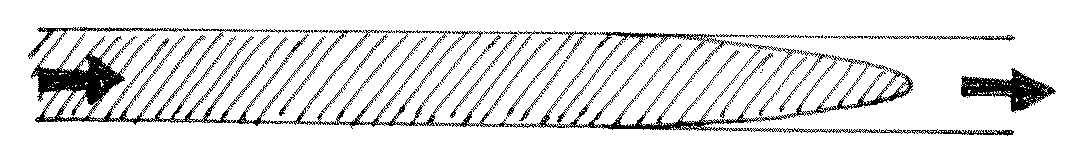
\includegraphics[width=\textwidth]{./figures/Topic2/Fig2-9.jpg}
	\caption{Parabolic blood flow based on Eq.~\ref{eqn2-7}.}
	\label{Fig2-10}
\end{figure}
By integrating the previous equation, we get Poiseuille’s law, which give the volume flow rate of a vessel of radius $R$ and length $L$, taking into account viscosity.
\begin{align}
\frac{dV}{dt} &= \int_0^R v(r) dA\nonumber\\
\frac{dV}{dt} &= \int_0^R v(r)\cdot d\left(\pi r^2\right)\nonumber\\
\frac{dV}{dt} &= \int_0^R v(r)\cdot 2\pi r dr\nonumber\\
\frac{dV}{dt} &= 2\pi \frac{\Delta P}{4\eta L}\int_0^R \left(rR^2 - r^3\right)dr\nonumber
\end{align}
\begin{equation}\label{eqn2-8}
\frac{dV}{dt} = \frac{\pi\Delta P R^4}{8\eta L}
\end{equation}
Note the fourth power dependence of flow rate on radius $R$.  Small changes in the diameter of a blood vessel lead to significant changes in the volume flow rate.  Our bodies take advantage of this sensitive dependence to control the blood supply to tissues. This is accomplished with the use of special muscle tissue surrounding blood vessels that contract or dilate to balance the local demand for blood.  
Thus far, we have considered only the laminar flow of blood, meaning that the fluid moves in smooth, parallel layers.  However, under certain conditions, the flow may become turbulent.  Viscous flow can become turbulent at high Reynold’s numbers.  Reynolds numbers are dimensionless and can be computed using the following equation:
\begin{equation}\label{eqn2-9}
{\rm Re} = \frac{\rho v d}{\eta}
\end{equation}
\[   {\rm flow} = \left\{
\begin{array}{ll}
      {\rm turbulent} & {\rm Re}\leq 3000 \\          
      {\rm unstable} & 2000 < {\rm Re} < 3000 \\
      {\rm laminar} & {\rm Re}\leq 2000 \\
\end{array} 
\right. \]
where $\rho$ is the density and $d$ is the diameter of the blood vessel.  Usually, Re must be greater than about 2000 before the flow becomes turbulent in a smooth vessel. However, turbulence can also be present at lower Reynolds numbers when the fluid passes through a narrowing or when branches into smaller vessels.

Blood flows into the aorta with an average speed of 32 cm/s.  Assuming the diameter of the artery is 2 cm, the viscosity of blood is 0.04 poise, and the density of blood is 1 g/cm$^3$, we estimate the Reynolds number to be 1600, a value critically close to the turbulent limit. Significant levels of turbulence are in fact generated within the aorta if the vessel is narrowed at some point, which can occur when a clot is present. Turbulence can also occur when an aortic valve cannot open fully, forcing the heart to pump blood at a higher velocity into the aorta. Turbulent flow produces a distinct sound that is known in the medical community as a murmur. This sound can be detected with a stethoscope.